\documentclass{standalone}
\usepackage{tikz}
\usetikzlibrary{patterns, positioning}


\begin{document}
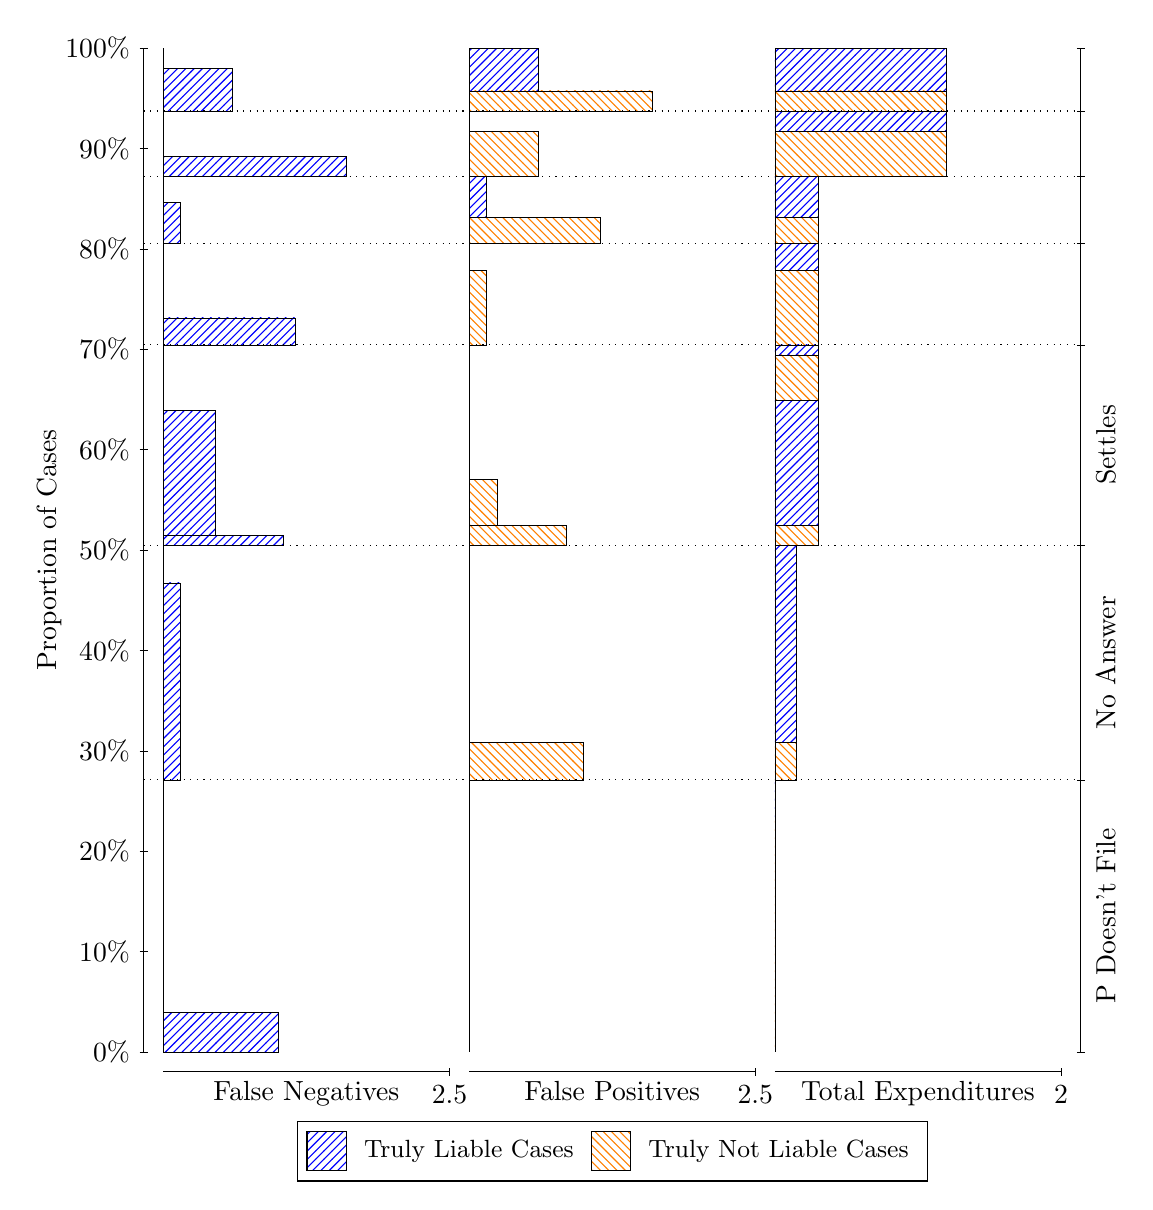
\begin{tikzpicture}
\draw[black, very thin] (1.5,1.75) -- (1.5,14.5);
\node[rotate=90, text=black, anchor=center] at (0.3, 8.125) {Proportion of Cases};
\draw[black, very thin] (1.45,1.75) -- (1.55,1.75);
\node[text=black, anchor=east] at (1.45, 1.75) {0\%};
\draw[black, very thin] (1.45,3.025) -- (1.55,3.025);
\node[text=black, anchor=east] at (1.45, 3.025) {10\%};
\draw[black, very thin] (1.45,4.3) -- (1.55,4.3);
\node[text=black, anchor=east] at (1.45, 4.3) {20\%};
\draw[black, very thin] (1.45,5.575) -- (1.55,5.575);
\node[text=black, anchor=east] at (1.45, 5.575) {30\%};
\draw[black, very thin] (1.45,6.85) -- (1.55,6.85);
\node[text=black, anchor=east] at (1.45, 6.85) {40\%};
\draw[black, very thin] (1.45,8.125) -- (1.55,8.125);
\node[text=black, anchor=east] at (1.45, 8.125) {50\%};
\draw[black, very thin] (1.45,9.4) -- (1.55,9.4);
\node[text=black, anchor=east] at (1.45, 9.4) {60\%};
\draw[black, very thin] (1.45,10.675) -- (1.55,10.675);
\node[text=black, anchor=east] at (1.45, 10.675) {70\%};
\draw[black, very thin] (1.45,11.95) -- (1.55,11.95);
\node[text=black, anchor=east] at (1.45, 11.95) {80\%};
\draw[black, very thin] (1.45,13.225) -- (1.55,13.225);
\node[text=black, anchor=east] at (1.45, 13.225) {90\%};
\draw[black, very thin] (1.45,14.5) -- (1.55,14.5);
\node[text=black, anchor=east] at (1.45, 14.5) {100\%};

\draw[black, very thin] (13.4,1.75) -- (13.4,14.5);
\draw[black, very thin] (13.35,1.75) -- (13.45,1.75);
\node[anchor=west] at (13.35, 1.75) {};
\draw[black, very thin] (13.35,5.2056) -- (13.45,5.2056);
\node[anchor=west] at (13.35, 5.2056) {};
\draw[black, very thin] (13.35,8.1874) -- (13.45,8.1874);
\node[anchor=west] at (13.35, 8.1874) {};
\draw[black, very thin] (13.35,10.731) -- (13.45,10.731);
\node[anchor=west] at (13.35, 10.731) {};
\draw[black, very thin] (13.35,12.018) -- (13.45,12.018);
\node[anchor=west] at (13.35, 12.018) {};
\draw[black, very thin] (13.35,12.866) -- (13.45,12.866);
\node[anchor=west] at (13.35, 12.866) {};
\draw[black, very thin] (13.35,13.7) -- (13.45,13.7);
\node[anchor=west] at (13.35, 13.7) {};
\draw[black, very thin] (13.35,14.5) -- (13.45,14.5);
\node[anchor=west] at (13.35, 14.5) {};

\draw[black, very thin, pattern color=blue, pattern=north east lines] (1.75,1.75) rectangle (3.2033,2.2495);
\draw[black, very thin, pattern color=orange, pattern=north west lines] (1.75,2.2495) rectangle (1.75,5.2056);
\draw[black, very thin, pattern color=blue, pattern=north east lines] (1.75,5.2056) rectangle (1.968,7.7064);
\draw[black, very thin, pattern color=orange, pattern=north west lines] (1.75,7.7064) rectangle (1.75,8.1874);
\draw[black, very thin, pattern color=blue, pattern=north east lines] (1.75,8.1874) rectangle (3.276,8.3146);
\draw[black, very thin, pattern color=blue, pattern=north east lines] (1.75,8.3146) rectangle (2.404,9.9013);
\draw[black, very thin, pattern color=orange, pattern=north west lines] (1.75,9.9013) rectangle (1.75,10.731);
\draw[black, very thin, pattern color=blue, pattern=north east lines] (1.75,10.731) rectangle (3.4213,11.073);
\draw[black, very thin, pattern color=orange, pattern=north west lines] (1.75,11.073) rectangle (1.75,12.018);
\draw[black, very thin, pattern color=blue, pattern=north east lines] (1.75,12.018) rectangle (1.968,12.537);
\draw[black, very thin, pattern color=orange, pattern=north west lines] (1.75,12.537) rectangle (1.75,12.866);
\draw[black, very thin, pattern color=blue, pattern=north east lines] (1.75,12.866) rectangle (4.0753,13.121);
\draw[black, very thin, pattern color=orange, pattern=north west lines] (1.75,13.121) rectangle (1.75,13.7);
\draw[black, very thin, pattern color=blue, pattern=north east lines] (1.75,13.7) rectangle (2.622,14.246);
\draw[black, very thin, pattern color=orange, pattern=north west lines] (1.75,14.246) rectangle (1.75,14.5);
\draw[black, very thin, pattern color=orange, pattern=north west lines] (5.6333,1.75) rectangle (5.6333,4.706);
\draw[black, very thin, pattern color=blue, pattern=north east lines] (5.6333,4.706) rectangle (5.6333,5.2056);
\draw[black, very thin, pattern color=orange, pattern=north west lines] (5.6333,5.2056) rectangle (7.0867,5.6866);
\draw[black, very thin, pattern color=blue, pattern=north east lines] (5.6333,5.6866) rectangle (5.6333,8.1874);
\draw[black, very thin, pattern color=orange, pattern=north west lines] (5.6333,8.1874) rectangle (6.8687,8.4415);
\draw[black, very thin, pattern color=orange, pattern=north west lines] (5.6333,8.4415) rectangle (5.9967,9.0176);
\draw[black, very thin, pattern color=blue, pattern=north east lines] (5.6333,9.0176) rectangle (5.6333,10.731);
\draw[black, very thin, pattern color=orange, pattern=north west lines] (5.6333,10.731) rectangle (5.8513,11.676);
\draw[black, very thin, pattern color=blue, pattern=north east lines] (5.6333,11.676) rectangle (5.6333,12.018);
\draw[black, very thin, pattern color=orange, pattern=north west lines] (5.6333,12.018) rectangle (7.3047,12.347);
\draw[black, very thin, pattern color=blue, pattern=north east lines] (5.6333,12.347) rectangle (5.8513,12.866);
\draw[black, very thin, pattern color=orange, pattern=north west lines] (5.6333,12.866) rectangle (6.5053,13.446);
\draw[black, very thin, pattern color=blue, pattern=north east lines] (5.6333,13.446) rectangle (5.6333,13.7);
\draw[black, very thin, pattern color=orange, pattern=north west lines] (5.6333,13.7) rectangle (7.9587,13.955);
\draw[black, very thin, pattern color=blue, pattern=north east lines] (5.6333,13.955) rectangle (6.5053,14.5);
\draw[black, very thin, pattern color=orange, pattern=north west lines] (9.5167,1.75) rectangle (9.5167,4.706);
\draw[black, very thin, pattern color=blue, pattern=north east lines] (9.5167,4.706) rectangle (9.5167,5.2056);
\draw[black, very thin, pattern color=orange, pattern=north west lines] (9.5167,5.2056) rectangle (9.7892,5.6866);
\draw[black, very thin, pattern color=blue, pattern=north east lines] (9.5167,5.6866) rectangle (9.7892,8.1874);
\draw[black, very thin, pattern color=orange, pattern=north west lines] (9.5167,8.1874) rectangle (10.062,8.4415);
\draw[black, very thin, pattern color=blue, pattern=north east lines] (9.5167,8.4415) rectangle (10.062,10.028);
\draw[black, very thin, pattern color=orange, pattern=north west lines] (9.5167,10.028) rectangle (10.062,10.604);
\draw[black, very thin, pattern color=blue, pattern=north east lines] (9.5167,10.604) rectangle (10.062,10.731);
\draw[black, very thin, pattern color=orange, pattern=north west lines] (9.5167,10.731) rectangle (10.062,11.676);
\draw[black, very thin, pattern color=blue, pattern=north east lines] (9.5167,11.676) rectangle (10.062,12.018);
\draw[black, very thin, pattern color=orange, pattern=north west lines] (9.5167,12.018) rectangle (10.062,12.347);
\draw[black, very thin, pattern color=blue, pattern=north east lines] (9.5167,12.347) rectangle (10.062,12.866);
\draw[black, very thin, pattern color=orange, pattern=north west lines] (9.5167,12.866) rectangle (11.697,13.446);
\draw[black, very thin, pattern color=blue, pattern=north east lines] (9.5167,13.446) rectangle (11.697,13.7);
\draw[black, very thin, pattern color=orange, pattern=north west lines] (9.5167,13.7) rectangle (11.697,13.955);
\draw[black, very thin, pattern color=blue, pattern=north east lines] (9.5167,13.955) rectangle (11.697,14.5);
\draw[black, dotted] (1.5,5.2056) -- (13.4,5.2056);
\draw[black, dotted] (1.5,8.1874) -- (13.4,8.1874);
\draw[black, dotted] (1.5,10.731) -- (13.4,10.731);
\draw[black, dotted] (1.5,12.018) -- (13.4,12.018);
\draw[black, dotted] (1.5,12.866) -- (13.4,12.866);
\draw[black, dotted] (1.5,13.7) -- (13.4,13.7);
\draw[black, very thin] (1.75,1.5) -- (5.3833,1.5);
\node[text=black, anchor=north] at (3.5667, 1.5) {False Negatives};
\draw[black, very thin] (5.3833,1.45) -- (5.3833,1.55);
\node[text=black, anchor=north] at (5.3833, 1.45) {2.5};

\draw[black, very thin] (5.6333,1.5) -- (9.2667,1.5);
\node[text=black, anchor=north] at (7.45, 1.5) {False Positives};
\draw[black, very thin] (9.2667,1.45) -- (9.2667,1.55);
\node[text=black, anchor=north] at (9.2667, 1.45) {2.5};

\draw[black, very thin] (9.5167,1.5) -- (13.15,1.5);
\node[text=black, anchor=north] at (11.333, 1.5) {Total Expenditures};
\draw[black, very thin] (13.15,1.45) -- (13.15,1.55);
\node[text=black, anchor=north] at (13.15, 1.45) {2};

\node[text=black, centered, rotate=90] at (13.72, 3.4778) {P Doesn't File};
\node[text=black, centered, rotate=90] at (13.72, 6.6965) {No Answer};
\node[text=black, centered, rotate=90] at (13.72, 9.4594) {Settles};





\draw (7.449999999999999,1.5) node[draw=none] (baseCoordinate) {};
\begin{scope}[align=center]
        \matrix[scale=0.5, draw=black, below=0.5cm of baseCoordinate, nodes={draw}, column sep=0.1cm]{
            \node[rectangle, draw, minimum width=0.5cm, minimum height=0.5cm, pattern color=blue, pattern=north east lines] {}; &
            \node[draw=none, font=\small, text=black] (B) {Truly Liable Cases}; &
            \node[rectangle, draw, minimum width=0.5cm, minimum height=0.5cm, pattern color=orange, pattern=north west lines] {}; &
            \node[draw=none, font=\small, text=black] (B) {Truly Not Liable Cases}; \\
            };
\end{scope}

\end{tikzpicture}
\end{document}